\documentclass[12pt,letterpaper,portrait,onecolumn,titlepage,twoside,
final,openany]{book}

\usepackage[left=1cm, right=2cm, top=2cm,bottom=2cm,bindingoffset=1cm]{geometry}
\usepackage{booktabs}
\usepackage{tabularx}
\usepackage[spanish]{babel}
\usepackage[export]{adjustbox}
\usepackage{listings}
\usepackage{color}
\usepackage{hyperref}
\usepackage{float}
\usepackage[T1]{fontenc}
\usepackage{lmodern}
\usepackage{datetime}
\usepackage{titletoc}% http://ctan.org/pkg/titletoc
\usepackage{pdfpages}

\titlecontents*{chapter}% <section-type>
  [0pt]% <left>
  {\addvspace{1em}}% <above-code>
  {\bfseries\chaptername\ \thecontentslabel\quad}% <numbered-entry-format>
  {}% <numberless-entry-format>
  {\bfseries\hfill\contentspage}% <filler-page-format>
  
\definecolor{mygreen}{rgb}{0,0.6,0}
\definecolor{mygray}{rgb}{0.5,0.5,0.5}
\definecolor{mymauve}{rgb}{0.58,0,0.82}

\lstset{ %
  backgroundcolor=\color{white},   % choose the background color; you must add \usepackage{color} or \usepackage{xcolor}
  basicstyle=\footnotesize,        % the size of the fonts that are used for the code
  breakatwhitespace=false,         % sets if automatic breaks should only happen at whitespace
  breaklines=true,                 % sets automatic line breaking
  captionpos=b,                    % sets the caption-position to bottom
  commentstyle=\color{mygreen},    % comment style
  deletekeywords={...},            % if you want to delete keywords from the given language
  escapeinside={\%*}{*)},          % if you want to add LaTeX within your code
  extendedchars=true,              % lets you use non-ASCII characters; for 8-bits encodings only, does not work with UTF-8
  frame=single,                    % adds a frame around the code
  keepspaces=true,                 % keeps spaces in text, useful for keeping indentation of code (possibly needs columns=flexible)
  keywordstyle=\color{blue},       % keyword style
  language=Octave,                 % the language of the code
  morekeywords={*,...},            % if you want to add more keywords to the set
  numbers=left,                    % where to put the line-numbers; possible values are (none, left, right)
  numbersep=5pt,                   % how far the line-numbers are from the code
  numberstyle=\tiny\color{mygray}, % the style that is used for the line-numbers
  rulecolor=\color{black},         % if not set, the frame-color may be changed on line-breaks within not-black text (e.g. comments (green here))
  showspaces=false,                % show spaces everywhere adding particular underscores; it overrides 'showstringspaces'
  showstringspaces=false,          % underline spaces within strings only
  showtabs=false,                  % show tabs within strings adding particular underscores
  stepnumber=2,                    % the step between two line-numbers. If it's 1, each line will be numbered
  stringstyle=\color{mymauve},     % string literal style
  tabsize=2,                       % sets default tabsize to 2 spaces
  title=\lstname                   % show the filename of files included with \lstinputlisting; also try caption instead of title
}

\renewcommand{\contentsname}{\'Indice}
\renewcommand{\figurename}{Diagramas}
\renewcommand{\listfigurename}{\'Indice de ilustraciones}
\renewcommand{\tablename}{Tablas}
\renewcommand{\listtablename}{\'Indice de tablas}

\newcommand{\head}[1]{\textnormal{\textbf{#1}}}
\begin{document}
\sloppy       %Para no cortar palabras junto con la librería hyphenat

\frontmatter
%% Este documento se realizó con el propósito de proporcionale a los estudiantes del CIDETEC un machote en latex de la tesis. Espero que les sirva de ayuda.
% Atte: Dr. Miguel Gabriel Villarreal Cervantes.
%*********************************************************************************************************
%*********************************************************************************************************
% Portada
\thispagestyle{empty}%

\begin{center}

\begin{tabular}[c]{ccc}
\hspace{-2cm}
\begin{tabular}[c]{r}

\includegraphics[height=1in,width=.8in]{Prefacio/Logo/logo_ipn.eps}
\end{tabular}
&
\begin{tabular}[c]{c}
\text{{\LARGE INSTITUTO POLITÉCNICO NACIONAL}}\\
\text{{\large Centro de Innovación y Desarrollo Tecnológico}}\\
\text{{\large  en Cómputo}}\\
\end{tabular}
&
\begin{tabular}[c]{l}

\includegraphics[height=1in,width=1in]{Prefacio/Logo/logo_cidetec.png}
\end{tabular}
\end{tabular}

\vspace{2cm}

{\large \textbf{TITULO} }

% No comentar Para colocar dos filas de t�tulo
%\bigskip
%{\large \textbf{M�s texto de t�tulo}}

\vspace{2cm}


{Tesis que para obtener el grado de}

\bigskip

\textbf{Maestro en Tecnología de Computo}

\bigskip

\vspace{2cm}

{Presenta}

\bigskip

{\large \textbf{xxxxxxxxxxxx}}


\vspace{2cm}


{Director(es)}

\bigskip

\textbf{xxxxxxxxxxxxxxxxxxxxxx}


\vspace{3cm}

México, D.F. \hspace{9.6cm} Junio del 2017.
%\today %Para colocar el d�a actual
\end{center}

%*********************************************************************************************************
%*********************************************************************************************************
% Dedicatoria
\newpage
\empty
\thispagestyle{empty}
\chapter*{\centerline{\Huge \textbf{Dedicatoria}}}
\pagenumbering{roman}
\vspace{4.5cm}
\begin{center}%
\begin{tabular}
[c]{l}%
\emph{xxxxx.}\\
\\
\emph{xxxxx.}\\
\\
\emph{xxxxxx }\\
\emph{xxxxxx}\\
\\
\emph{xxxx}\\
\\
\emph{xxxxxx}\\
\emph{xxxxx}\\
\\


\end{tabular}
\end{center}

%*********************************************************************************************************
%*********************************************************************************************************
% Agradecimientos
%*********************************************************************************************************
%*********************************************************************************************************
\newpage
\empty
\thispagestyle{empty}
\chapter*{\centerline{\Huge \textbf{Agradecimientos}}}

\bigskip


\emph{Se agradece al Consejo Nacional de Ciencia y Tecnología (CONACYT)...}\\

\bigskip
\emph{A mi familia.}\\
\emph{A mi familia...}

\bigskip
\emph{A mis asesores...}


%Para los estudiantes del Dr. Villarreal Colocar lo siguiente para el caso del año 2015 para posteriores años favor de preguntarme.


%*********************************************************************************************************
%*********************************************************************************************************
% Resumen
%\newpage
%\empty
%\thispagestyle{empty}
%\chapter*{\centerline{\Huge \textbf{Resumen}}}
%En este trabajo de investigación se propone xxxxxx.\\
%
%
%xxxxxxx.
%
%
%%*********************************************************************************************************
%%*********************************************************************************************************
%% Resumen
%\newpage
%\empty
%\thispagestyle{empty}
%\chapter*{\centerline{\Huge \textbf{Abstract}}}
%In this research work a xxxxx.\\
%
%
%xxxxxx.

%*********************************************************************************************************
%*********************************************************************************************************
% Acronimos
\newpage
\empty
\thispagestyle{empty}
%\chapter*{\centerline{\Huge \textbf{Lista de acr�nimos}}}
\chapter*{{\Huge \textbf{Lista de acrónimos}}}

\begin{tabular}{ll}
  \hline
  % after \\: \hline or \cline{col1-col2} \cline{col3-col4} ...
	RMR:	& Robot Móvil con Ruedas  			\\
	RMO:	& Robot Móvil Omnidireccional		\\
  \hline
\end{tabular}

%*********************************************************************************************************
%*********************************************************************************************************
% Tabla de contenido
\newpage
\empty
\thispagestyle{empty}
\pdfbookmark{\contentsname}{Contents} %Pone los marcadores en el pdf. Se debe compilar con: dvi->ps, ps->pdf
\tableofcontents

%*********************************************************************************************************
%*********************************************************************************************************
% Tabla de figuras
\newpage
\empty
\thispagestyle{empty}
\listoffigures

%*********************************************************************************************************
%*********************************************************************************************************
% Tabla de figuras
\newpage
\empty
\thispagestyle{empty}
\listoftables
\newpage
\empty
%\thispagestyle{empty}  %Para la tesis, Quitar el comentario
% Este documento se realizó con el propósito de proporcionale a los estudiantes del CIDETEC un machote en latex de la tesis. Espero que les sirva de ayuda.
% Atte: Dr. Miguel Gabriel Villarreal Cervantes.
%*********************************************************************************************************
%*********************************************************************************************************
% Portada
\thispagestyle{empty}%

\begin{center}

\begin{tabular}[c]{ccc}
\hspace{-2cm}
\begin{tabular}[c]{r}
	
\includegraphics[height=1in,width=.8in]{Prefacio/Logo/logo_ipn.eps}
\end{tabular}
&
\begin{tabular}[c]{c}
\text{{\LARGE INSTITUTO POLITÉCNICO NACIONAL}}\\
\text{{\large CENTRO DE INOVACI\'{O}N Y DESARROLLO}}\\
\text{{\large TECNOL\'{O}GICO EN C\'{O}MPUTO }}\\
\end{tabular}
&
\begin{tabular}[c]{l}
	
\includegraphics[height=1in,width=1in]{Prefacio/Logo/logo_cidetec.png}
\end{tabular}
\end{tabular}



\vspace{2cm}

{\large \textbf{Generador de Macros Automático} }

% No comentar Para colocar dos filas de título
%\bigskip
%{\large \textbf{Más texto de título}}

\vspace{2cm}


{Tesis que para obtener el grado de}

\bigskip

\textbf{Maestro en Tecnología de Cómputo}

\bigskip

\vspace{2cm}

{Presenta}

\bigskip

{\large \textbf{Ricardo González Tello}}

\vspace{2cm}


{Directores}

\bigskip

\textbf{Dr. Mauricio Olguin Carbajal}

\textbf{M. en C. Patricia Pérez Romero}

\vspace{3cm}

México, D.F. \hspace{9.6cm} Junio del 2017.
%\today %Para colocar el día actual
\end{center}



%*********************************************************************************************************
%*********************************************************************************************************
% Tabla de contenido
\newpage
\empty
\thispagestyle{empty}
\pdfbookmark{\contentsname}{Contents} %Pone los marcadores en el pdf. Se debe compilar con: dvi->ps, ps->pdf
\tableofcontents

%*********************************************************************************************************
%*********************************************************************************************************
% Tabla de figuras
\newpage
\empty
\thispagestyle{empty}
\listoffigures

%*********************************************************************************************************
%*********************************************************************************************************
% Tabla de figuras
\newpage
\empty
\thispagestyle{empty}
\listoftables
\newpage
\empty
%\thispagestyle{empty} 
\decimalpoint
\mainmatter

%%=========================================
\chapter{Introducción}\label{cap1}
%\setcounter{secnumdepth}{4}
%=========================================



Como nos ha marcado la experiencia, la computadora al igual que cualquier otra
 máquina fue diseñada para facilitar la vida de las personas con las tareas
 repetitivas, ya sea acelerando o automatizando tareas, así mismo se ha llegado
 a un punto en la operación de la computadora en la que se realizan tareas de
 forma mecanizada ya que no hay variantes en estas.  

Los desarrolladores de software han contribuido a la automatización de estas
 tareas, sin embargo, cuando el software no es específico para una persona
 sino para un sector de la población, las necesidades llegan a ser variadas
 de un usuario a otro lo que genera un software con múltiples funciones de las
 cuales cada usuario usa un conjunto diferente esto es, por lo tanto,
 mientras más genérico se quiere hacer un software, más complicado será es su
 uso. 

Algunos de los desarrollos enfocados a la automatización de acciones humanas
 con las variantes involucradas en el mundo real principalmente son 
 aplicaciones de la robótica, sin embargo, las soluciones propuestas también
 pueden ser enfocadas a un ambiente virtual.

La propuesta presentada va enfocada al apoyo de las personas con acceso a la
 computadora, pero que debido a sus capacidades físicas no puede usar el equipo
 con la misma agilidad que una persona con todas sus facultades. Estas son las
 Personas con Movilidad Reducida(PRM), que principalmente, por cuestiones
 laborales tienen que trabajar con una computadora y que por su discapacidad se
 les dificulta el uso de la misma.

Por lo tanto, en este trabajo de investigación se propone desarrollar un sistema
 que permita el monitoreo de las acciones del usuario realizadas en una
 computadora personal (PC, Personal Computer) y obtener la secuencia de acciones
 frecuentes para su posterior reproducción.

\section{Justificación}
A nivel mundial, la discapacidad va en aumento dado que la población está
 envejeciendo y son pocos los programas privados y gubernamentales que apoyan a
 este grupo de personas\cite{OrganizacionMundialdelaSalud2011}. 
 Con referencia a los datos obtenidos del Censo de Población
 y Vivienda de 2010 era poco más del 5\% de la Población de México la que
 presentaba algún tipo de discapacidad, pero se puede apreciar que esta cifra va
 en aumento ya que en la Encuesta Nacional de Ingresos y Gasto de los Hogares
 (ENIGH) de 2012 fue el 6.6\% el porcentaje de la población la que tenía alguna
 discapacidad\cite{Milosavljevic2014}.
 

%Falta Escribir

 
La Organización Mundial de la Salud (OMS) y el Banco Mundial
\cite{OrganizacionMundialdelaSalud2011} proponen una
 estrategia de colaboración entre el sector privado y gubernamental para
 rehabilitar e incorporar a la sociedad a las personas discapacitadas y así
 poder aprovechar el potencial de toda esta gente.Algunas de estas propuestas
 tienen por objetivo proporcionar accesibilidad en los servicios convencionales
 , por ejemplo transporte y educación, así como adiestrar a los servidores
 públicos, para que las personas sean tratadas con los cuidados necesarios.
 
\section{Planteamiento del problema}
Con base en lo mencionado previamente, se puede apreciar que la población de
 Personas con Movilidad Reducida(PRM) va en aumento en México y con el uso de
 la computadora como algo imprescindible en la actualidad sobre todo en el
 sector laboral 2, la discapacidad de estas personas puede representar un
 obstáculo en su desarrollo laboral.
\section{Propuesta de trabajo}

Como un apoyo a las personas cuya discapacidad representa un obstáculo para
 interactuar de manera ágil y precisa con las computadoras de escritorio, se
 plantea desarrollar un sistema de reconocimiento de patrones con la capacidad
 reproducir las acciones que tengan mayor incidencia de uso. 
 
Para lo que se plantea utilizar una estructura de datos en árbol, en la cual
 se van a almacenar los movimientos del teclado y ratón que el usuario realice,
 para posteriormente cuantificar las incidencias de cada rama, esto estregara
 las secuencias útiles. Una vez detectada se le solicitara al usuario un nombre
 para esta secuencia por el cual pueda ser invocada posteriormente.
\section{Objetivo general} 
Diseñar y desarrollar un software que defina a partir de un periodo de tiempo
 determinado el conjunto de acciones con mayor incidencia de uso por un usuario
 realizadas en una computadora por un usuario, para su uso posterior.

\section{Objetivos específicos}
\begin{itemize}
  \item Desarrollar del sistema para la captura de acciones, tanto del  ratón
  como del teclado.
  \item Propuesta, creación e implementación de árbol.
  \item Obtener una muestra de las acciones realizadas con el teclado y el 
  ratón por un usuario en una computadora.
  \item Diseñar y desarrollar el algoritmo para la determinación de tareas
  repetitivas.
\end{itemize}


\section{Metodología}
Con el propósito de desarrollar y lograr los objetivos propuestos en el presente trabajo de investigación, se plantearon siguientes metas:
\section*{Metas}
\begin{itemize}
  \item Investigación de sistemas similares.
  \item Recopilación de resultados de sistemas similares.
  \item Desarrollo del sistema  de captura de datos.
  \item Obtención de los datos de ejemplo.
  \item Desarrollo del Sistema de procesamiento de datos.
  \item Realizar pruebas del sistema.
  \item Realizar un análisis comparativo de los resultados.
\end{itemize}
%Salto de pagina
%\pagebreak

\section{Cronograma de actividades}

\begin{figure}[h]
\centering
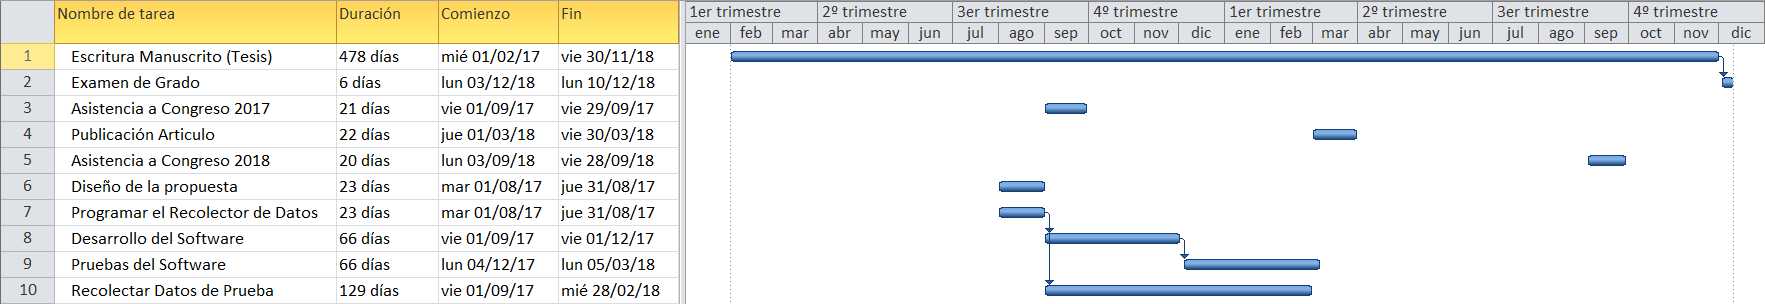
\includegraphics[width=1.0\columnwidth]{./CapituloI/Imagenes/Cronograma.PNG}
\end{figure}
% Este documento se realizó con el propósito de proporcionale a los estudiantes
del CIDETEC un machote en latex de la tesis. Espero que les sirva de ayuda.
% Atte: Dr. Miguel Gabriel Villarreal Cervantes.
%*****************************************************************************
%*****************************************************************************
% Capítulo I
\chapter{Introducción \label{cap1}}

La computadora al igual que cualquier otra máquina fue diseñada para facilitar
la vida de las personas, ya sea acelerando o facilitando el trabajo realizado.
Actualmente hay tareas que se realizan en la computadora y se hacen de forma
mecanizada ya que no hay variantes en estas. 

Por mencionar algunas de las herramientas existentes  para la automatización
este tipo de tareas se tienen las siguientes:

Macros: son un conjunto de instrucciones que el fabricante del software ha
colocado para agilizar manejo de este; sin embargo, el usuario tiene  que
aprender cómo utilizarlas, por ejemplo, una combinación de teclas. También
existen opciones para crear macros personalizadas, ya sea por una opción que
da el fabricante o con software de terceros…

El capítulo \ref{cap1} 

En \cite{RolandSiegwart+IllanNourbakhsh},


Por lo tanto en este trabajo de investigación se propone, como un problema ....


\section{Justificación}
A nivel mundial, la discapacidad va en aumento dado que la población está
envejeciendo y son pocos los programas privados y gubernamentales que apoyan a
este grupo de personas. Con referencia a los datos obtenidos Censo de Población
 y Vivienda de 2010 era poco más del 5\% de la Población de México la que
 presentaba algún tipo de discapacidad, pero se puede apreciar que esta cifra va
 en aumento ya que en la Encuesta Nacional de Ingresos y Gasto de los Hogares
 (ENIGH) de 2012 fue el 6.6\% el porcentaje de la población la que tenía alguna
 discapacidad.
 
 
La Organización Mundial de la Salud (OMS) y el Banco Mundial proponen una
 estrategia de colaboración entre el sector privado y gubernamental para
 rehabilitar e incorporar a la sociedad a las personas discapacitadas y así
 poder aprovechar el potencial de toda esta gente.
 
 
Algunas de estas propuestas tienen por objetivo proporcionar accesibilidad en
 los servicios convencionales, por ejemplo transporte y educación, así como
 adiestrar a los servidores públicos, para que las personas sean tratadas con
 los cuidados necesarios.
 
 
Como un apoyo a las personas que por su discapacidad presentan dificultad para
 interactuar de manera ágil y precisa con las computadoras de escritorio, se
 plantea desarrollar un sistema de reconocimiento de patrones con la capacidad
 reproducir las acciones que tengan mayor incidencia de uso.

\section{Planteamiento del problema}
Con base en lo mencionado previamente, se puede apreciar que la población de
 Personas con Movilidad Reducida(PRM) va en aumento en México y con el uso de
 la computadora como algo imprescindible en la actualidad sobre todo en el
 sector laboral 2, la discapacidad de estas personas puede representar un
 obstáculo en su desarrollo laboral.



\section{Objetivo general} 
Diseñar y desarrollar un software que defina a partir de un periodo de tiempo
 determinado el conjunto de acciones con mayor incidencia de uso por un usuario
 realizadas en una computadora por un usuario, para su uso posterior.

\section{Objetivos específicos}
\begin{itemize}
  \item Desarrollar del sistema para la captura de acciones, tanto del  ratón
  como del teclado.
  \item Obtener una muestra de las acciones realizadas con el teclado y el 
  ratón por un usuario en una computadora.
  \item Diseñar y desarrollar el algoritmo para la determinación de tareas
  repetitivas.
\end{itemize}


\section{Metodología}
Con el propósito de desarrollar y lograr los objetivos propuestos en el presente trabajo de investigación, se plantearon siguientes metas:
\section*{Metas}
\begin{itemize}
  \item[I] Investigación de sistemas similares.
  \item[II] Recopilación de resultados de sistemas similares.
  \item[III] Desarrollo del sistema  de captura de datos.
  \item[IV] Obtención de los datos de ejemplo.
  \item[V] Desarrollo del Sistema de procesamiento de datos.
  \item[VI] Realizar pruebas del sistema.
  \item[VII] Realizar comparativa de los resultados.
\end{itemize}





\section{Cronograma de actividades}



\begin{table}[h]
\centering
%EndExpansion
%

\begin{tabular}{|c|c|c|c|c|c|}
\hline
\multicolumn{6}{|c|}{Periodo 2013/02}\tabularnewline
\hline
\hline
Metas & Ago & Sep & Oct & Nov & Dic\tabularnewline
\hline
I & X & X & X & X & X\tabularnewline
\hline
II & X & X & X & X & \tabularnewline
\hline


\end{tabular}

\caption{Cronograma de Actividades I}
\label{reglasI}
\end{table}%
%EndExpansion



\begin{table}[h]
\centering
%EndExpansion
%

\begin{tabular}{|c|c|c|c|c|c|c|}
\hline
\multicolumn{7}{|c|}{Periodo 2014/01}\tabularnewline
\hline
\hline
Metas & Ene & Feb & Mar & Abr & May & Jun\tabularnewline
\hline
I & X & X & X & X & X & X\tabularnewline
\hline
III &  & X &  &  &  & \tabularnewline
\hline
IV.I & X & X & X & X & X & X\tabularnewline
\hline
V & X & X & X &  &  & \tabularnewline
\hline
VI &  & X & X &  &  & \tabularnewline
\hline


\end{tabular}
%

\caption{Conograma de Actividades II}
\label{reglasII}
\end{table}%



\begin{table}[h]
\centering
%EndExpansion
%

\begin{tabular}{|c|c|c|c|c|c|}
\hline
\multicolumn{6}{|c|}{Periodo 2014/02}\tabularnewline
\hline
\hline
Metas & Ago & Sep & Oct & Nov & Dic\tabularnewline
\hline
I & X & X &  &  & \tabularnewline
\hline
IV.II & X & X & X & X & X\tabularnewline
\hline
VII &  &  & X & X & \tabularnewline
\hline
VIII &  &  &  & X & X \tabularnewline
\hline
IX & X &  &  &  & \tabularnewline
\hline
X & X & X & X & X & X\tabularnewline
\hline
XV &  &  & X & X & X\tabularnewline
\hline
\end{tabular}
%

\caption{Conograma de Actividades III}
\label{reglasIII}
\end{table}%




\begin{table}[h]
\centering
%EndExpansion
%

\begin{tabular}{|c|c|c|c|c|c|c|}
\hline
\multicolumn{7}{|c|}{Periodo 2015/01}\tabularnewline
\hline
\hline
Metas & Ene & Feb & Mar & Abr & May & Jun\tabularnewline
\hline
I & X & X &  &  &  & \tabularnewline
\hline
XI & X & X & X & X &  & \tabularnewline
\hline
XII &  & X & X & X & X & \tabularnewline
\hline
XIII &  &  & X & X & X & \tabularnewline
\hline
XIV &  &  &  &  &  & X\tabularnewline
\hline
XV & X & X & X &  &  & \tabularnewline
\hline
\end{tabular}
%

\caption{Conograma de Actividades IV}
\label{reglasIV}
\end{table}% 






%%=========================================
\chapter{ Marco Teorico \label{cap2}}
%=========================================
 %Para la tesis

%%=========================================
\chapter{Capitulo III \label{cap3}}
%=========================================

\section{Teoría de árboles}
En términos matemáticos un árbol es un grafo $T$ el cual se puede definir de
 la siguiente forma\cite{SUSANNAS.EPP2012}:

\begin{itemize}
	\item ``Un grafo se llama árbol si y solo si, está libre de circuitos y
	 es conexo.''
	\item ``Un vértice de grado 1 en $T$ se denomina un vértice terminal (o
	 una hoja).''
	\item ``Un vértice de grado superior a 1 en $T$ es un vértice interno (o
	 un vértice de rama).''
\end{itemize}

Los arboles son muy usados en la actualidad ya que permiten  darle sentido a
 la información contenida, gracias a la asociatividad, parentización y
 prioridad que este permite de manera implícita. Entre sus usos múltiples en
 el área de la informática se pueden destacar los  siguientes; relaciones
 entre módulos de programación, arboles de decisión en inteligencia artificial
 y representaciones gramáticas\cite{gutierrez1999estructuras}.  

Una forma de ver a un árbol puede ser como un solo nodo, esté recibe el nombre
 de  nodo raíz, al cual se le puede enraizar un sinfín de arboles lo que da
 origen  a un árbol con otras características, dependiendo del resultado se le
 puede clasificar en alguno de los modelos existentes, por ejemplo; árbol 
 general o árbol binario\cite{gutierrez1999estructuras}. 

El árbol general es un modelo con una cantidad indeterminada de nodos hijos,
 mientras que el árbol binario es un caso particular del árbol general ya que
 este tiene la característica de tener siempre en cada nodo 2 nodos hijos como
 máximo, cabe mencionar que este es uno de los modelos a mas usados, así como
 el ultimo caso mencionado, hay arboles que tienen una cantidad fija de nodos
 hijos, de manera general estos son llamados arboles n-arios
 \cite{gutierrez1999estructuras}. %Para la tesis

%%==================================================================================
\chapter{Capitulo XXX}
\label{cap4}
%\setcounter{secnumdepth}{5}
%==================================================================================
 %Para la tesis

%%=========================================
\chapter{Resultados \label{cap5}}
%========================================= %Para la tesis

%%=========================================
\chapter{Conclusiones y perspectivas \label{cap6}}
%=========================================

\cite{RolandSiegwart+IllanNourbakhsh} %Para la tesis

\bibliographystyle{IEEEtran}
\bibliography{Bibliografia}

%%*********************************************************************************************************
%*********************************************************************************************************
% Apéndices
\appendix

\chapter{Apendice XXX \label{Apen:A}}



\chapter{Publicaciones \label{ApenD}}
A continuación se presenta una lista de los artículos publicados en congresos de arbitraje nacional que se realizaron durante el periodo en que se realizo la tesis de maestría


 %Para la tesis

%\include{Apendice/Apendice/ApendiceC/ApendiceC}
\end{document}